\section{Clase de un instrumento}

Se define como ``límite de error'' al mayor error absoluto que comete un instrumento en algún punto de la escala y que puede ser tanto positivo como negativo. Este error absoluto máximo se debe a la suma de pequeños errores sistemáticos que actúan simultáneamente: imperfección de la escala, del índice, falta de constancia de algún parámetro interviniente de la cupla, etc.
\[
  E_\text{max} = \text{Límite de error}
\]
Se define ``clase de un instrumento'' al límite de error referido al alcance por cien:
\[
  c=\frac{E_\text{max}}{\text{Alcance}}\cdot 100\%
\]
Esta expresión, nos permite conocer para un valor dado de la clase el límite de error \(E_\text{max}\):
\[
  \pm E_\text{max} = \frac{c\text{Alcance}}{100}
\]
Es decir que si efectuamos una lectura coincidente con una división exacta de la escala tenemos un error límite denominado ``error por clase'' e igual a:
\[
  \pm E_\text{max}
\]
Mencionamos ``división exacta de la escala'' para no introducir el error de estimación. Para comprender el concepto de clase, hagamos el siguiente planteo: Supongamos que comparamos el instrumento -cuya clase se desconoce- con otro patrón o exacto; es evidente que para cada medición habrá una diferencia entre valor medido y valor real (probable) del instrumento patrón:
\[
  E=V_m-V_r
\]
En algún punto de la escala aparecerá un \(E_\text{máximo}\), definido como límite de error y el que se toma en cuenta para el cálculo de la clase. Ahora bien, cuando nosotros realizamos una medición cualquiera, puede ocurrir que el error absoluto cometido sea menor que el error absoluto límite (pues éste puede estar en otro punto de la escala). Sin embargo desconocemos en que lugar o división se encuentra \(e_\text{max}\) y como en el campo de las mediciones se adopta siempre un criterio pesimista, ante la incertidumbre se debe tomar el error límite, como un error absoluto máximo y constante para cualquier punto de la escala.

Los instrumentos de clase entre 0,05 y 0,1 son los de mayor exactitud y son usados como patrones de referencia para la calibración y contraste de otros instrumentos, o bien para ensayos de laboratorio donde se requiera una exactitud elevada.

Los instrumentos de clase 0,2 hasta 0,5 se usan en ensayos normales de laboratorio y contraste de instrumentos de una clase de exactitud por lo menos cinco veces mayor. Los instrumentos de clase mayor a 1 son construidos exclusivamente para instalar en tableros o paneles, casi siempre de escala vertical o bien para instrumentos portátiles donde no se requieren mediciones de buena exactitud.

La clase de un instrumento es establecida por el fabricante. Nosotros podemos verificar si el instrumento ``está en clase''. Para el establecimiento de la clase, debe ajustarse a normas establecidas y utilizando patrones de laboratorio.

\subsubsection*{Determinación de la clase por el fabricante}

El fabricante diseña un instrumento tratando de cumplir ciertas condiciones:
\begin{enumerate}
  \item Temperatura ambiente constante, entre \qtyrange{20}{25}{\degreeCelsius} denominado temperatura de calibración.
  \item Reducción de campos magnéticos externos (menor que 5 Oesterd). %No se que es oesterd
  \item Para un instrumento de corriente alterna, excitación sinusoidal y frecuencia determinada.
  \item Posición normal de trabajo (horizontal, vertical, etc.).
\end{enumerate}

Una vez cumplidas estas condiciones se debe disponer un instrumento patrón, de alcance en general similar al instrumento a calibrar. Se deben fijar previamente los puntos cardinales, es decir el ``cero'' y ``fondo de escala''. Para fijar el cero se lo hace mecánicamente, sin excitación y el punto fondo de escala con excitación. Se fijan valores particulares en el patrón en cifras enteras para determinar puntos intermedios de la escala, pudiendose tomar 5 a 10; consecuentemente mediante el conocimiento de la ley de distribución de la misma se han de trazar las divisiones restantes hasta completar la totalidad de la escala que en general oscila de 100 a 150 divisiones.
% Me siento medio tonto, pero me he perdido un poco con este parrafo ¿A que se refiere con ley de distribución de la misma?

Esto último sería para los instrumentos prototipos. Para los instrumentos de tipo serie, por razones económicas ya se cuenta con la escala impresa.

Luego lo que se suele hacer es un contraste, que es una verificación de la clase. Para ello se toman divisiones exactas y se determinan las diferencias con el patrón.

\subsection{Quebrada de corrección}

Los errores absolutos obtenidos por diferencias con el patrón, cambiados de signo son los denominados valores de corrección. Se puede entonces trazar una gráfica en función del valor medido, que se denomina ``quebrada de corrección''. Es típica la forma dentada de la curva. Entre los valores de corrección de los puntos contiguo se efectúa una interpolación lineal. En algunos casos -instrumentos de hierro móvil, por ejemplo, la corriente de excitación utilizada en la comprobación debe aumentarse en forma continua -sin inversión- hasta llegar a fondo de escala. Luego se repite la verificación con corriente decreciente desde fondo de escala hasta ``cero''. Los valores de corrección se forman en base a los valores medios entre calibración creciente y decreciente. Las diferencias entre valores crecientes y decrecientes son indicativos de la calidad del instrumento, especialmente sobre el rozamiento, reacciones elásticas, etc.

Estas quebradas de corrección son generalmente realizadas por el mismo fabricante y entregadas al usuario, en aquellos instrumentos de buena calidad, de los utilizados en laboratorios. Por supuesto, en los instrumentos de serie, estas curvas no se entregan y las mediciones realizadas son acotadas teniendo en cuenta el límite de error obtenido a partir del índice de clase.

\subsection{Valor fiduciario}
%¿Qué es fiduciario?

Es el valor convencional para determinar la exactitud del instrumento. Para un instrumento con cero lateral, el valor correspondiente al límite superior del campo de medida. Por ejemplo un amperímetro de \qtyrange{0}{100}{\ampere}, el valor fiduciario es \qty{100}{\ampere}. %¿No sería lo mismo que el alcance?

Para un instrumento de cero intermedio: la suma de los valores absolutos correspondientes a cada uno de los límites. Por ejemplo un milivoltímetro con campo de medida de \qtyrange{-15}{35}{\milli\volt}, el valor convencional es de \qty{50}{\milli\volt}.

Para un instrumento con cero retirado -no figura en el cuadrante- el valor convencional corresponde al límite superior del campo de medida. Por ejemplo para un voltímetro de \qtyrange{180}{260}{\volt}, el valor fiduciario es \qty{260}{\volt}-.

Para un frecuencímetro, sea a indice ó a lengüetas, el valor corresponde el límite superior. Por ejemplo para un frecuencímetro de campo de medida \qtyrange{40}{60}{\hertz}, el valor convencional es de \qty{60}{\hertz}. Téngase en cuenta que la norma C.E.I. define como campo de indicación a la gama de valores del grandor medido que corresponde al recorrido total del índice sobre la escala. Mientras que el campo de medidas corresponde a la parte de la escala que en las condiciones de referencia pueden hacerse las lecturas con la exactitud que implica la clase del instrumento.

Los extremos del campo de medida quedan definidos por ``límite inferior y superior''. La norma determina que el límite del campo de medida debe estar identificado sobre el cuadrante sin ambigüedad.

\subsection{Cota de error}

Habíamos visto que la expresión de la clase era:
\[
  c=\pm\frac{E_\text{max}}{\text{Alcance}}\cdot 100
\]
El límite de error 
\[
  E_\text{max} = \frac{c\text{Alcance}}{100}
\]
Veamos el siguiente caso: se obtuvieron dos mediciones de una misma magnitud con dos instrumentos diferentes, cuyas características son las siguientes:
\begin{enumerate}
  \item \textbf{Voltímetro 1}: Alcance \qty{30}{\volt}; \qty{150}{\div}; $c=1$
  \item \textbf{Voltímetro 2}: Alcance \qty{30}{\volt}; \qty{150}{\div}; $c=0,2$
\end{enumerate}
El error límite para cada uno de los instrumentos será:
\[
  E_\text{max1}=\pm\qty{0.3}{\volt}
  \quad \text{y}\quad
  E_\text{max2}=\pm\qty{0.06}{\volt}
\]
Suponiendo ahora que la lectura en ambos instrumentos coinciden en una división exacta $\alpha=\qty{50}{\div}$, tendremos
\begin{itemize}
  \item Para el voltímetro 1, $V_m=10\pm\qty{0.3}{\volt}$.
  \item Para el voltímetro 2, $V_m=10\pm\qty{0.06}{\volt}$.
\end{itemize}
Este caso solamente tomando el error de clase, no considerando ningún otro error en la medición, como puede ser el error ``debido al método'', etc.

El error relativo de indicación será para cada voltímetro:
\[
  e_1=3\% \quad \text{y} \quad e_2=0.6\%
\]
Conclusión: si tomamos el voltímetro 1 diremos que para este instrumento de clase igual a uno, el límite de error es $\pm 3\%$; significa que se trata de un voltímetro de características funcionales y constructivas tales que los diferentes errores instrumentales sistemáticos se comportan de manera que funcionando en condiciones normales de uso el error absoluto máximo no será superior a \qty{0.3}{\volt} en cualquier parte de la escala.
% Muy lindo ejemplo, pero creo que es algo repetitivo. Si puedes lee la unidad 1 en el repositorio de github, notaras que esta definición ya está en el glosario.

\subsection{Condición más favorable para una medición}

El error relativo porcentual de indicación o de clase está dado por la expresión 
\[
  e_i\% = \pm \frac{E_\text{max}}{V_m} 100
\]
Como $E_\text{max}$ lo suponemos constante
\[
  e_i\% = \pm \frac{K}{V_m} 100 % esto me parece innecesario
\]

% Esto no lo borres, me ha servido mucho
De la curva de la figura \ref{fig:error_en_funcion_alcance} vemos que el error relativo de la indicación va siendo menor a medida que el valor medido esté próximo al alcance del instrumento. Es por ello que se recomienda que la magnitud a medir esté dentro de un valor próximo al alcance del instrumento. % Esto me parece un dato bastante importante. Podríamos hacer un gráfico con tikz (usando axis) de 1/x para representar este comportamiento ¿no?
% A continuación dejo un esquema de esta situación
\begin{figure}[!ht]
  \centering
  \begin{tikzpicture}[scale=0.7]
    \begin{axis}[
        axis lines = middle,
        xlabel = {$V_m$},
        ylabel = {$e_i\%$},
        domain = 0.3:8,
        ymin = 0, ymax = 10,
        xmin = 0, xmax = 11,
        samples = 100,
        width=10cm, height=8cm,
        restrict y to domain=0:10,
        xticklabel=\empty,
        yticklabel=\empty,
    ]
        \addplot [
            red,
            thick,
        ] {12/x};

      \draw[black,dotted] (8,2) -- (8, 0) node[above left,black]{\scriptsize{Alcance}};
      \draw[black,dotted] (1,10) -- (1, 0);
    \end{axis}
  \end{tikzpicture}
  \caption{}
  \label{fig:error_en_funcion_alcance}
  % Importante: ignora la escala numérica, es un esquema hipotético adimensional.
\end{figure}
Lo razonable es efectuar mediciones comprendidas en el último tercio de la escala.

\subsection{Escalas no lineales}

Todo lo anterior es válido cuando la ley del instrumento es lineal. Veamos ahora que ocurre con el error relativo de indicación en aplicaciones no tan comunes como en instrumentos con escala alineal dilatada (escala cuadrática) o escala alineal comprimida (escala logarítmica). Las expresiones de las cotas de error y sus correspondientes errores relativos de indicación serán:

\subsubsection*{a. Escala alineal dilatada}
\[
  \alpha=K_1 X_m^2
\]
diferenciando:
\[
  d\alpha=2K_1 X_m dX
\]
Pasando de diferenciales a incrementos finitos:
\[
  \Delta \alpha_\text{max} = 2K_1 X_m \Delta X_\text{max} \implies \Delta X_\text{max}= \frac{\Delta \alpha}{2K_1 X_m}
\]
Pero
\[
  \Delta \alpha_\text{max} = \frac{c \text{Alcance}}{100} \quad \text{y}\quad \Delta X_\text{max} = \frac{c \text{Alcance}}{200 K_1 X_m}
\]
Luego
\[
  e_1 = \frac{\Delta X_\text{max}}{X_\text{med}}= \frac{K_2}{X_m}
\]

\subsubsection*{b. Escala alineal comprimida}

Tomando como ejemplo la escala logarítmica:
\[
  \alpha = K_1 \ln X_m
\]
diferenciando
\[
  d\alpha = K_1 \frac{1}{X_m}dX
\]
Pasando a incrementos finitos:
\begin{gather*}
  \Delta \alpha_\text{max} = \frac{K\Delta X_\text{max}}{X_m} \\ 
  \Delta X_\text{max} = \frac{X_m \Delta_\text{max}}{K_1}=\frac{X_m c \text{Alcance}}{100 K_1} = K_2 X_m
\end{gather*}
pero,
\[
  e_i = \frac{\Delta X_\text{max}}{X_m}= \frac{K_2X_m}{X_m} = K_2
\]
Entonces, $e_i=K_2=\text{constante}$. Para el instrumento de escala uniforme el error relativo varía según una hipérbola equilátera. Un análisis comparativo del uso de los tres tipos de instrumentos para un rango determinado de mediciones, arrojaría los siguientes resultados (figura \ref{fig:error_no_lineal}).
\begin{figure}[!ht]
  \centering
  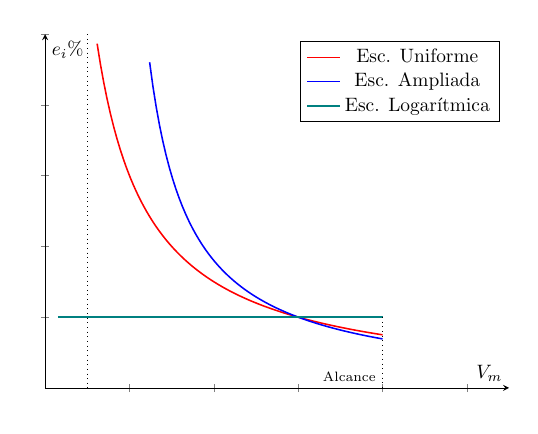
\begin{tikzpicture}[scale=0.7]
    \begin{axis}[
        axis lines = middle,
        xlabel = {$V_m$},
        ylabel = {$e_i\%$},
        domain = 0.3:8,
        ymin = 0, ymax = 10,
        xmin = 0, xmax = 11,
        samples = 100,
        width=10cm, height=8cm,
        restrict y to domain=0:10,
        xticklabel=\empty,
        yticklabel=\empty,
    ]
        \addplot [
            red,
            thick,
        ] {12/x};
        \addlegendentry{Esc. Uniforme};
        \addplot [
            blue,
            thick,
        ] {9/(x-1.5)};
        \addlegendentry{Esc. Ampliada};
        \addplot [
          teal,
          thick,
        ] {2};
        \addlegendentry{Esc. Logarítmica};

      \draw[black,dotted] (8,2) -- (8, 0) node[above left,black]{\scriptsize{Alcance}};
      \draw[black,dotted] (1,10) -- (1, 0);
    \end{axis}
  \end{tikzpicture}
  \caption{}
  \label{fig:error_no_lineal}
  % Importante: ignora la escala numérica, es un esquema hipotético adimensional.
  % tampoco borres esta figura, me guía bastante.
\end{figure}

Si la condición es obtener lecturas con escasa influencia del error relativo de indicación se observa que el primer tercio de la escala debería descartarse.

El segundo tercio, el instrumento de escala uniforme aventaja al de escala ampliada. Finalmente la última parte de la escala el menor error corresponde al instrumento con escala ampliada. Este tipo de instrumento es utilizado en aquellos casos en que la variación de lectura permanente varía muy poco -por ejemplo un voltímetro que indique la tensión a la salida del generador de un grupo electrógeno-, en esta parte de la escala el aparato posee buena resolución. Para escala logarítmica, el error relativo se mantiene constante. Este tipo de escala es útil para medir magnitudes de luz y sonido.

\subsection{Campo nominal de referencia y campo de utilización}

La norma C.E.I. establece para cada parámetro de referencia en la calibración de un instrumento un margen de variación, para el cual el aparato debe mantenerse en clase.

Así por ejemplo tomando el parámetro temperatura la norma establece una tolerancia de $\pm \qty{1}{\degreeCelsius}$ para instrumentos de clase 0,1; 0,2; 0,5 y un margen de $\pm\qty{2}{\degreeCelsius}$ para los de clase 1,0; 1,5; 2,5. Tomemos por ejemplo un instrumento de clase igual a uno, con una temperatura de referencia de \qty{25}{\degreeCelsius}, la tolerancia de la temperatura será y por lo tanto entre los \qty{23}{\degreeCelsius} y \qty{27}{\degreeCelsius} y manteniendo el resto de los parámetros en las condiciones de referencia, el instrumento cometerá errores de indicación dentro de la banda permitida por el índice de la clase.

El límite del campo nominal de utilización fijado por la norma es $\pm\qty{10}{\degreeCelsius}$, esto significa que para el margen que va entre \qtyrange{15}{23}{\degreeCelsius} y entre \qtyrange{27}{35}{\degreeCelsius} deben esperarse errores relativos de indicación no superiores a dos veces la clase del instrumento. Para otros factores de influencia (frecuencia, campos magnéticos externos, etc.) las normas establecen los respectivos márgenes de variación de acuerdo a la calidad del instrumento.

\subsection{Propagación de errores límites}

Las mediciones pueden clasificarse en mediciones directas y mediciones indirectas. Las mediciones directas son aquellas en que el valor de la magnitud a medir surge directamente de la lectura en un instrumento; por el contrario las mediciones indirectas son aquellas en que la medida surge como una función matemática que relaciona dos o más funciones o medidas directas. Por ejemplo la potencia consumida por una resistencia $R$, medida a través de un voltímetro y amperímetro se determina por la función matemática: $P = UI$.

Ahora bien, cada una de éstas mediciones directas estarán afectadas de sus correspondientes errores absolutos límites. De la propagación de ellos surgirá el error límite de la medición indirecta.

En general el valor $w$ medido indirectamente es función de:
\[
  w=f(u,v)
\]
siendo $u$ y $v$ variables independientes, que pueden ser aquellas que medimos directamente por ejemplo con instrumentos indicadores, o bien aquellos que corresponden a elementos que integran el circuito de medida como resistores, de los que conocemos los valores nominales dados por el fabricante, junto con que respectivas tolerancias o errores.

Si calculamos el diferencial $dw$:
\[
  dw = \frac{\partial w}{\partial u}du + \frac{\partial w}{\partial v}dv
\]
Esta expresión sigue siendo aproximadamente válida, si en lugar de diferenciales consideramos incrementos finitos, si estos con suficientemente pequeños:
\[
  \Delta w = \frac{\partial w}{\partial u}\Delta u + \frac{\partial w}{\partial v}\Delta v
\]
siendo $\Delta w$ el error absoluto límite de $w$, $\Delta u$ el de $u$ y $\Delta v$ el de $v$.

Esta expresión nos da directamente el incremento (error) $\Delta w$ de la cantidad que se mide indirectamente en función de los incrementos (errores $\Delta u$ y $\Delta v$ ) de las variables medidas directamente y vale tanto para ``errores sistemáticos'', ``fortuitos'' o límites.

Si $\Delta u$ y $\Delta v$ son errores absolutos límites se adopta un criterio pesimista quedando la expresión de la siguiente forma:
\[
  \pm E_w = \pm \left[ \left\lvert \frac{\partial w}{\partial u} \right\rvert E_u + 
  \left\lvert \frac{\partial w}{\partial v} \right\rvert E_v\right]
\]
El error relativo será en este caso 
\[
  \pm e_w = \pm \frac{E_w}{w}= \pm \frac{1}{w}\left[ \left\lvert \frac{\partial w}{\partial u} \right\rvert E_u + 
  \left\lvert \frac{\partial w}{\partial v} \right\rvert E_v\right]
\]
